%!TEX root = ../../../exa-ma-d7.1.tex
\section{Software: CGAL}
\label{sec:WP1:CGAL:software}

\begin{table}[h!]
    \centering
    { \setlength{\parindent}{0pt}
    \def\arraystretch{1.25}
    \arrayrulecolor{numpexgray}
    {\fontsize{9}{11}\selectfont
    \begin{tabular}{!{\color{numpexgray}\vrule}p{.4\textwidth}!{\color{numpexgray}\vrule}p{.6\textwidth}!{\color{numpexgray}\vrule}}
        \rowcolor{numpexgray}{\rule{0pt}{2.5ex}\color{white}\bf Field} & {\rule{0pt}{2.5ex}\color{white}\bf Details} \\
        \rowcolor{white}\textbf{Consortium} & \begin{tabular}{l}
Inria\\
\end{tabular} \\
        \rowcolor{numpexlightergray}\textbf{Exa-MA Partners} & \begin{tabular}{l}
Inria CA\\
\end{tabular} \\
        \rowcolor{white}\textbf{Contact Emails} & \begin{tabular}{l}
christos.georgiadis@inria.fr\\
pierre.alliez@inria.fr\\
\end{tabular} \\
        \rowcolor{numpexlightergray}\textbf{Supported Architectures} & \begin{tabular}{l}
CPU Only\\
\end{tabular} \\
        \rowcolor{white}\textbf{Repository} & \href{https://github.com/CGAL}{https://github.com/CGAL} \\
        \rowcolor{numpexlightergray}\textbf{License} & \begin{tabular}{l}
OSS:: GPL v*\\
OSS:: LGPL v*\\
\end{tabular} \\
        \rowcolor{white}\textbf{Bottlenecks roadmap} & \begin{tabular}{l}
B10 - Scientific Productivity\\
B11 - Reproducibility and Replicability of Computation\\
B6 - Data Management\\
B7 - Exascale Algorithms\\
\end{tabular} \\
        \bottomrule
    \end{tabular}
    }}
    \caption{WP1: CGAL Information}
\end{table}

\subsection{Software Overview}
\label{sec:WP1:CGAL:summary}

%\textbf{WP1 description from white paper:}

The focus of WP1 is on revisiting discretization methodologies, particularly for large-scale models,
that incorporate multiple phenomena and process couplings. The main tasks include mesh generation, adaptive refinement, 
and the development of finite element frameworks. Additionally, emphasis is placed on creating parallelization 
strategies that can significantly enhance scalability and overall performance of the algorithms. 

CGAL will serve as the foundational library providing the geometric computing building blocks to develop some of the 
relevant discretization algorithms. The focus will be on robustness, geometric fidelity and performance. 
CGAL already provides a variety of algorithms for the manipulation of geometric data.
In particular, we will focus on two components for mesh generation given a wide range of inputs: 3D mesh generation \cite{jamin_cgalmesh_2015,alliez_3d_2024} and 3D alpha wrapping \cite{portaneri_alpha_2022,alliez_3d_2024-1}.

The 3D mesh generation package relies upon filtering and refinement of 3D Delaunay triangulations, ensuring the creation of high-quality isotropic tetrahedral meshes for complex geometric domains. 
The algorithm guarantees that the mesh conforms accurately to the input surface, while respecting user-defined constraints on parameters such as size of elements, boundary approximation, and element quality. In addition to mesh generation, CGAL provides refinement strategies that adaptively improve mesh quality, while ensuring that the resulting structure remains optimized as the domain's complexity grows.



Nowadays, real-world input data come from a variety of sources and sensors, and are often ill-defined for accurate representation of the domain, 
such as a unorganized 3D point clouds obtained by scanning an entire city. 3D data are commonly acquired through measurements followed by shape reconstruction, 
or generated through imperfect automated processes. Consequently, this data can exhibit a wide range of defects, including gaps, 
missing elements, self-intersections, degeneracies like zero-volume structures, and non-manifold features, making accurate 
and reliable geometric processing a challenge. The 3D Alpha Wrapping component offers a way to deal with this kinds of data by providing an algorithm that creates a valid 3D triangulation that strictly encloses the input. The algorithm offers unconditional robustness to the input, i.e., the output is guaranteed to be a watertight and orientable surface triangle mesh, regardless of the input quality.

Table~\cref{tab:WP1:CGAL:features} records a summary of the software features relevant to the work package which are briefly discussed.

\begin{table}[h!]
    \centering
    { 
        \setlength{\parindent}{0pt}
        \def\arraystretch{1.25}
        \arrayrulecolor{numpexgray}
        {
            \fontsize{9}{11}\selectfont
            \begin{tabular}{!{\color{numpexgray}\vrule}p{.25\linewidth}!{\color{numpexgray}\vrule}p{.6885\linewidth}!{\color{numpexgray}\vrule}}
    
    \rowcolor{numpexgray}{\rule{0pt}{2.5ex}\color{white}\bf Features} &  {\rule{0pt}{2.5ex}\color{white}\bf Short Description }\\ 
    
\rowcolor{white}    unstructured mesh & 3D Delaunay Mesh Generation, 3D Alpha Wrapping \\
\end{tabular}
        }
    }
    \caption{WP1: CGAL Features}
    \label{tab:WP1:CGAL:features}
\end{table}


\subsection{Parallel Capabilities}
\label{sec:WP1:CGAL:performances}

%\begin{itemize}
%    \item describe the parallel programming  environment : MPI, OpenMP, CUDA, OpenACC, etc.
%    \item describe the parallel computation environment: type of architecture and super computer used.
%    \item describe the parallel capabilities of the software
%    \item \textbf{Scalability:} Describe the general scalability properties of the software
%    \item \textbf{Integration with Other Systems:} Describe how the software integrates with other numerical libraries in the Exa-MA framework.
%\end{itemize}

CGAL does not yet offer parallel implementation with distributed memory. Nevertheless, its 3D mesh generation package supports multi-core shared-memory parallelism, via Intel's Thread Building Blocks (TBB) library.

The 3D Alpha Wrapping algorithm is not yet parallelized and runs on a single thread.

For future numerical experiments involving parallel algorithms, 
we will use a DELL precision workstation equipped with two 26-core Intel Xeon Gold 6230R CPUs clocked at 2.10 GHz, providing a total count of 104 threads, running on a 64-bit architecture, with 512 GB of RAM.

%\url{https://doc.cgal.org/latest/Mesh_3/index.html#Mesh_3ParallelAlgorithms}


\subsection{Initial Performance Metrics}
\label{sec:WP1:CGAL:metrics}



%This section provides a summary of initial performance benchmarks performed in the context of WP1. It ensures reproducibility by detailing input/output datasets, benchmarking tools, and the results. All data should be publicly available, ideally with a DOI for future reference.
%
%\begin{itemize}
%    \item \textbf{Overall Performance:} Summarize the software's computational performance, energy efficiency, and scalability results across different architectures (e.g., CPU, GPU, hybrid systems).
%    \item \textbf{Input/Output Dataset:} Provide a detailed description of the dataset used for the benchmark, including:
%        \begin{itemize}
%            \item Input dataset size, structure, and format (e.g., CSV, HDF5, NetCDF).
%            \item Output dataset format and key results.
%            \item Location of the dataset (e.g., GitHub repository, institutional repository, or open access platform).
%            \item DOI or permanent link for accessing the dataset.
%        \end{itemize}
%    \item \textbf{open-data Access:} Indicate whether the datasets used for the benchmark are open access, and provide a DOI or a direct link for download. Where applicable, highlight any licensing constraints.
%    \item \textbf{Challenges:} Identify any significant bottlenecks or challenges observed during the benchmarking process, including data handling and computational performance.
%    \item \textbf{Future Improvements:} Outline areas for optimization, including dataset handling, memory usage, or algorithmic efficiency, to address identified challenges.
%\end{itemize}

We now provide initial performance metrics of the two relevant discretization algorithms. The benchmarks have been performed as part of the packages release in CGAL.

%\subsubsection{Benchmark \#1}
%\begin{itemize}
%    \item \textbf{Description:} Briefly describe the benchmark case, including the problem size, target architecture (e.g., CPU, GPU), and the input data. Mention the specific goals of the benchmark (e.g., testing scalability, energy efficiency).
%    \item \textbf{Benchmarking Tools Used:} List the tools used for performance analysis, such as Extrae, Score-P, TAU, Vampir, or Nsight, and specify what metrics were measured (e.g., execution time, FLOPS, energy consumption).
%    \item \textbf{Input/Output Dataset Description:}
%        \begin{itemize}
%            \item \textbf{Input Data:} Describe the input dataset (size, format, data type) and provide a DOI or link to access it.
%            \item \textbf{Output Data:} Specify the structure of the results (e.g., memory usage, runtime logs) and how they can be accessed or replicated.
%            \item \textbf{Data Repository:} Indicate where the data is stored (e.g., Zenodo, institutional repository) and provide a DOI or URL for accessing the data.
%        \end{itemize}
%    \item \textbf{Results Summary:} Include a summary of key metrics (execution time, memory usage, FLOPS) and their comparison across architectures (e.g., CPU, GPU).
%    \item \textbf{Challenges Identified:} Describe any bottlenecks encountered (e.g., memory usage, parallelization inefficiencies) and how they impacted the benchmark.
%\end{itemize}


\subsubsection{Benchmark \#1 - 3D Alpha Wrapping serial}


The 3D alpha wrapping does not offer parallelization at its current stage of development. We provide in~\cref{WP1::CGAL::aw3} the complexity analysis from~\cite{portaneri_alpha_2022} on a single 3D model (fan model, available in GrabCad) and using a single thread. 
The plots shows that the computational time correlates well with the output mesh complexity (number of triangles).


\begin{figure}[htb]
    \centering
    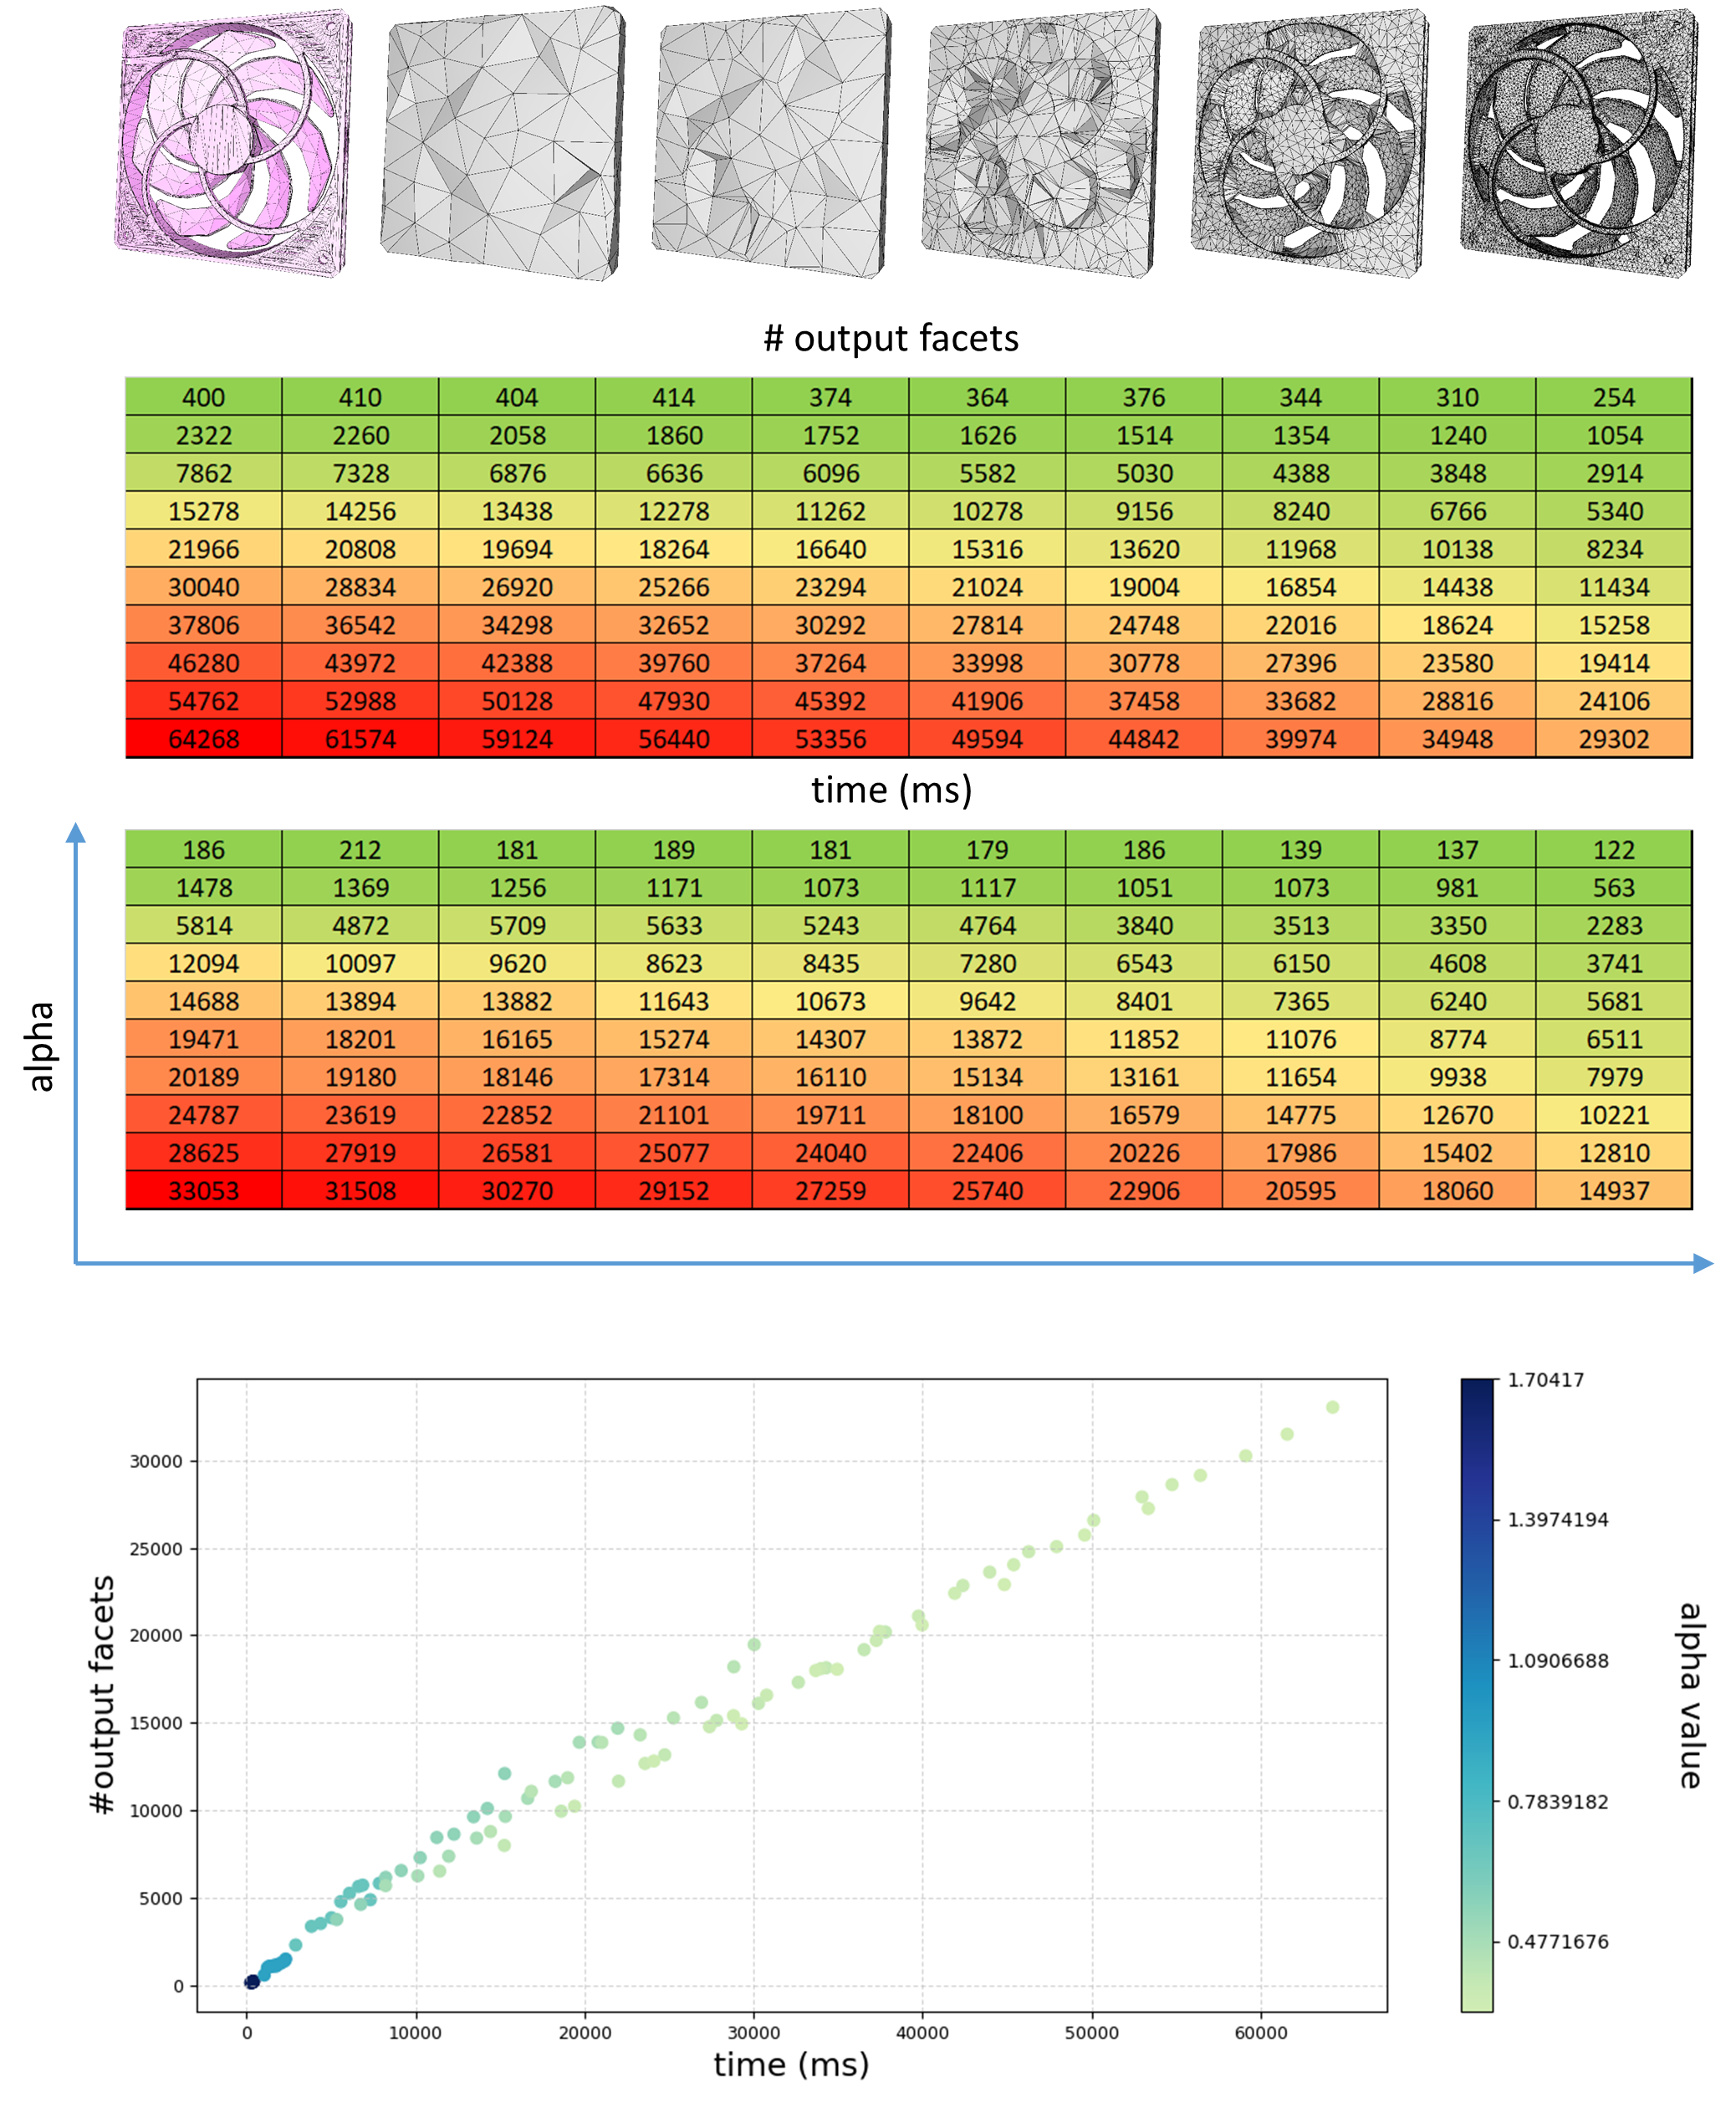
\includegraphics[width=0.6\textwidth]{graphics/cgal/fan.png} 
    \caption{Output complexity and time against alpha/offset parameters.
\textbf{Top:} Input fan model, and few output meshes shown for increasing alpha parameter. \textbf{Middle top:} Complexity of the output mesh in number of triangle
facets. Middle bottom: Computational time in ms. \textbf{Bottom:} Computational time against complexity of the output mesh. Each dot corresponds to one above combination of alpha/offset parameters.}
\label{WP1::CGAL::aw3}
\end{figure}



\subsubsection{Benchmark \#2 - 3D Mesh Generation parallel}


The speed-up charts in~\cref{WP1::CGAL::mg3parallel} are generated using the parallel version of the 3D meshing algorithm and were obtained from the 3D mesh generation reference manual \cite{alliez_3d_2024}. 
The machine used is a PC running Windows 7 64-bits with two 6-core Intel Xeon CPU X5660 clocked at 2.80 GHz with 32GB of RAM. 
The program has been compiled with Microsoft Visual C++ 2012, in Release mode.
The models used for this benchmark are publicly available in the CGAL Git repository, specifically in the 'demo' folder.


\begin{figure}[htb]
    \centering
    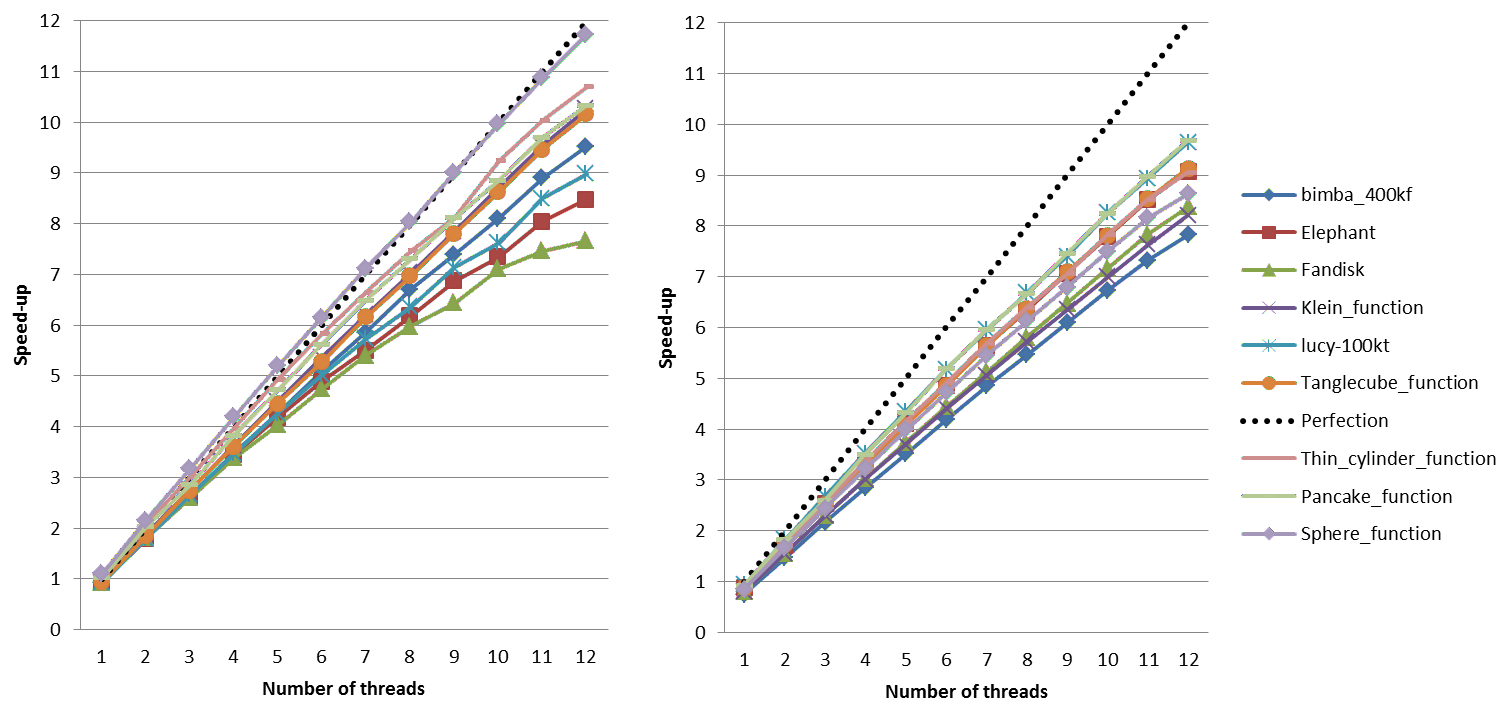
\includegraphics[width=0.6\textwidth]{graphics/cgal/refinement_speedup.png} 
    \caption{Facet refinement speed-up (left) and cell refinement speed-up (right), compared to the sequential version of the algorithm.}
    \label{WP1::CGAL::mg3parallel}
\end{figure}


\subsection{12-Month Roadmap}
\label{sec:WP1:CGAL:roadmap}

%In this section, describe the roadmap for improving benchmarks and addressing the challenges identified. This should include:
%\begin{itemize}
%    \item \textbf{Data Improvements:} Plans for improving input/output data management, including making datasets more accessible and ensuring reproducibility through open-data initiatives.
%    \item \textbf{Methodology Application:} Implementation of the benchmarking methodology proposed in this deliverable to streamline reproducibility and dataset management.
%    \item \textbf{Results Retention:} Plans to maintain benchmark results in a publicly accessible repository with appropriate metadata and documentation, ensuring long-term usability.
%\end{itemize}



Our current efforts focus on developing a feature-preserving, reduced-complexity version of the 3D Alpha Wrapping algorithm.
The goal is two-fold: on the one hand it will ensure that the domain's features (such as corners, cusps or sharp creases) are accurately represented in the output. On the other hand, obtaining a feature preserving mesh also offers a means to obtain an output with a reduced complexity (number of vertices) required to enclose the input domain, thus offering an improvement in performance even for the serial version of the algorithm. 
In practice this means that the feature-preserving 3D Alpha Wrapping will complement a parsimonious variant.
In our context, parsimony translates into minimizing the number of vertices to accurately represent the input domain by keeping 
the geometric discrepancy (measured as the Hausdorff distance between the output surface and the input) bounded.
Proper identification of the domain's features during meshing will allow us to directly connect these features over planar and sufficiently 
smooth regions without generating unnecessary vertices, thereby achieving a satisfactory balance between accuracy and simplicity.


% cite https://hal.science/hal-03380593/file/2021216131.pdf christos-todo 
Furthermore, more scalable parallelization schemes are currently under development in CGAL by GeometryFactory and IGN (Institut National de l'Information Géographique et Forestière), utilizing the distributed memory paradigm and a generic framework. Following the generic approach of CGAL, we can hopefully use them on existing algorithms, such as the 3D Alpha Wrapping. 
Nevertheless, designing a distributed version of a mesh generation algorithm is a non-trivial task that requires addressing several significant technical challenges.
During mesh generation, the domain evolves dynamically, making it difficult to maintain a balanced decomposition with an even number of elements across different subdomains.
As a result, a careful load-balancing strategy is essential.
Additionally, new vertices generated by separate threads must not coincide or be positioned too closely. Maintaining conflict-free areas between different subdomains may become a significant bottleneck, especially as the number of processors increases.


In~\cref{tab:WP1:CGAL:bottlenecks}, we briefly discuss the bottleneck roadmap associated to the software and relevant to the present work package.

\begin{table}[h!]
    \centering
    
    

    \centering
    { 
        \setlength{\parindent}{0pt}
        \def\arraystretch{1.25}
        \arrayrulecolor{numpexgray}
        {
            \fontsize{9}{11}\selectfont
            \begin{tabular}{!{\color{numpexgray}\vrule}p{.25\linewidth}!{\color{numpexgray}\vrule}p{.6885\linewidth}!{\color{numpexgray}\vrule}}
    
    \rowcolor{numpexgray}{\rule{0pt}{2.5ex}\color{white}\bf Bottlenecks} &  {\rule{0pt}{2.5ex}\color{white}\bf Short Description }\\ 
    
\rowcolor{white}    B10 - Scientific Productivity & Well documented examples should be provided along with our developed algorithms, as they already exist for 3D Mesh Generation and 3D Alpha Wrapping packages of CGAL.  \\
\rowcolor{numpexlightergray}    B11 - Reproducibility and Replicability of Computation & The codes and data will be publicly available and open-source. \\
\rowcolor{white}    B6 - Data Management & Benchmark scripts will be available, using publicly available large databases of geometric models. \\
\rowcolor{numpexlightergray}    B7 - Exascale Algorithms & Challenges regarding distributed mesh generation involve dynamic load-balancing and scalability with increasing number of threads. \\
\end{tabular}
        }
    }
    \caption{WP1: CGAL plan with Respect to Relevant Bottlenecks}
    \label{tab:WP1:CGAL:bottlenecks}
\end{table}


%B10 Scientific Productivity : Provide scientists with tools to use exascale systems
%productively, including program development, application execution, input
%preparation, output collection, and result analysis.

%B11 Reproducibility and Replicability of Computation : Ensure that research results are
%reproducible and that data and codes are provided so others can re-obtain the
%same results.

%B6 Data Management : Develop software that handles massive amounts of data,
%addressing both offensive I/O (e.g., data analysis and compression) and defensive
%I/O (e.g., fault tolerance).

%B7 Exascale Algorithms : Redesign algorithms to improve scalability by reducing
%communication, avoiding or hiding synchronization, and enhancing computational
%efficiency on accelerators.
